\chapter{Redukcja częstotliwości używając JK}

\section{Budowa układu}

\begin{itemize}
    \item Korzystając z układu JK (TTL 7493 (\ref{link:7493})) należało zbudować układ dzielący (redukujący) częstotliwość przez dwa.
        \begin{figure}[H]
            \centering
            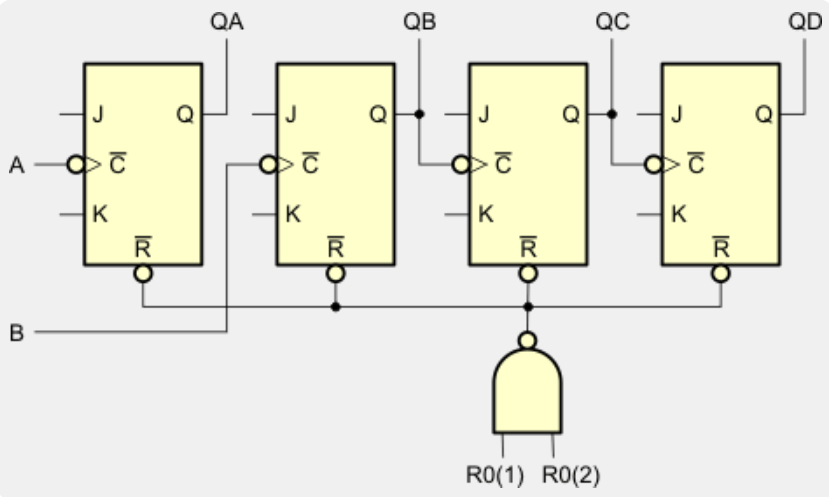
\includegraphics[width=0.7\textwidth]{img/schemes/logic_scheme_7943.png}
            \caption{Schemat logiczny układu 7493}
            \label{JK_dzielenie:schemat_logiczny}
        \end{figure}
        \begin{figure}[H]
            \centering
            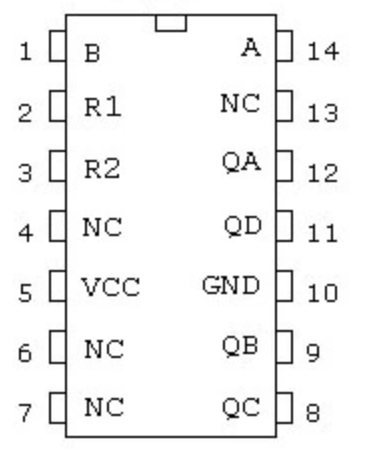
\includegraphics[width=0.3\textwidth]{img/schemes/7493_pins.png}
            \caption{Piny TTL 7493}
            \label{JK_dzielenie:piny}
        \end{figure}
    \item Korzystając ze schematu logicznego układu 7493 (\ref{JK_dzielenie:schemat_logiczny}) oraz przebiegu czasowego licznika 4-bitowego (\ref{licznik:przebieg}) zbudowano układ. Zgodnie z przebiegem czasowym licznika częstotliwość równa połowie wejściowym znajduje się na pinie QA (12).
    \item Sygnał wejściowy wpięto do wejścia A (pin 14), wyjściowy z QA (pin 12) z którego wychodzi sygnał do oscyloskopu.
    \item Clear/Reset ($\overline{R}$) generowany jest poprzez bramke NAND o wejściach R1, R2 (piny 2,3). Do wejść resetu wpięto impulsator.
        \begin{figure}[H]
            \centering
            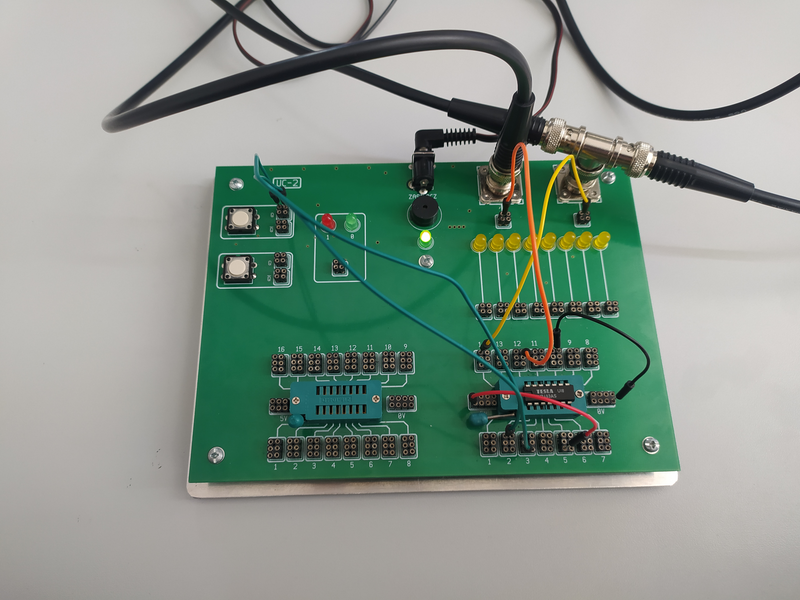
\includegraphics[width=\textwidth]{img/dzielenie/1653500524827_scaled.png}
            \caption{Zbudowany układ dzielący częstotliwość}
            \label{JK_dzielenie:zbudowany_uklad}
        \end{figure}
        
        \begin{figure}[H]
            \centering
            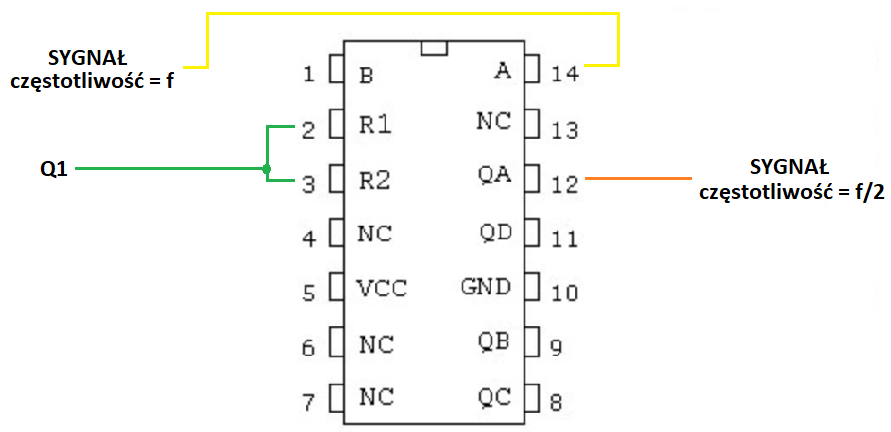
\includegraphics[width=\textwidth]{img/schemes_w_pins/dzielenie_w_pins.png}
            \caption{Schemat z połączonymi pinami}
            \label{JK_dzielenie:schemat_z_pinami}
        \end{figure}
\end{itemize}

\pagebreak

\section{Pomiary}

\begin{itemize}
    \item Korzystając z pomiaru za pomocą funkcji wbudowanych w oscyloskopie zmierzono częstotliwość wejściowego sygnału oraz wyjściowego sygnału.
        \begin{figure}[H]
            \centering
            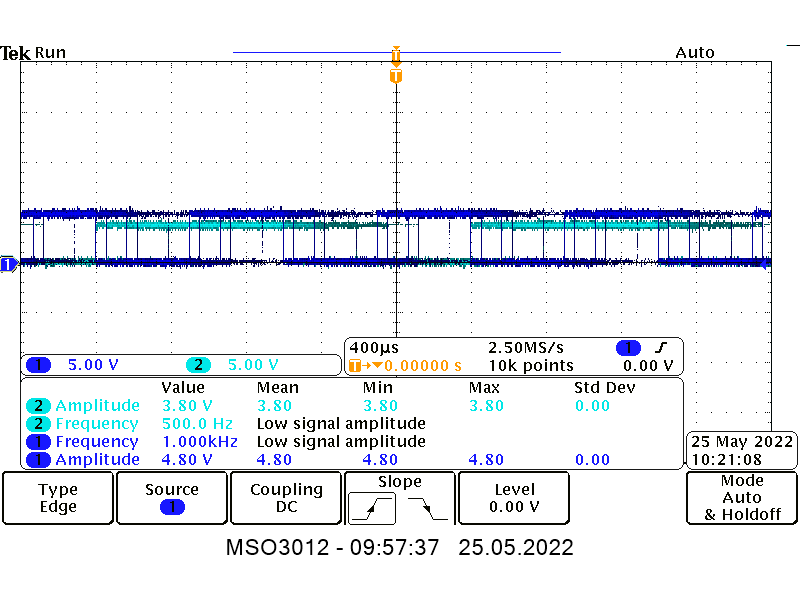
\includegraphics[width=0.8\textwidth]{img/dzielenie/polowa_okresu.png}
            \label{JK_dzielenie:wskazanie oscyloskopu}
        \end{figure}
    \item Na wejście (kanał 1) podano sygnał prostokątny o wartościach:
        \begin{center}
            $f_{we}$ = \textbf{1kHz}
            $U_{low}$ = \textbf{0V}
            $U_{high}$ = \textbf{5V}
        \end{center}
    \item Częstotliwość sygnału wyjściowego (kanał 2) jest dwa razy mniejsza od częstotliwości sygnału wejsciowego (kanał 1) ($\dfrac{500Hz}{1kHz}=\dfrac{1}{2}$).
    \item Układ działa \textbf{poprawnie}.
\end{itemize}